\documentclass[
titlepage=firstiscover,
bibliography=totoc,
captions=tableheading,
]{scrartcl}

\usepackage[aux]{rerunfilecheck}



\usepackage{polyglossia}
\usepackage[autostyle]{csquotes}
\setmainlanguage{german}
\setotherlanguages{english, french}

\usepackage{microtype}

\usepackage{amsmath}
\usepackage{amssymb}
\usepackage{mathtools}

\usepackage{fontspec}

\usepackage[
  style=alphabetic,
]{biblatex}
\addbibresource{main.bib}

\usepackage[
math-style=ISO,
bold-style=ISO,
sans-style=italic,
nabla=upright,
partial=upright,
]{unicode-math}

\usepackage[
  locale=DE,
  separate-uncertainty=true,
  per-mode=symbol-or-fraction,
]{siunitx}

\sisetup{
locale=DE,
per-mode=symbol-or-fraction}

\usepackage[unicode]{hyperref}
\usepackage{bookmark}

\usepackage{graphicx}
\graphicspath{{build/}}

\usepackage{caption, booktabs}

\usepackage{grffile}
\usepackage{subcaption}
\usepackage{float}

\usepackage{xfrac}


\title{SMD: Blatt 4}
\author{
  Sophie Bork
  \texorpdfstring{
    \\
    \href{mailto:sophie.bork@udo.edu}{sophie.bork@udo.edu}
  }{}
  \texorpdfstring{\and}{, }
  Simon Schulte
  \texorpdfstring{
    \\
    \href{mailto:simon.schulte@udo.edu}{simon.schulte@udo.edu}
  }{}
  \texorpdfstring{\and}{, }
  Michael Windau
  \texorpdfstring{
    \\
    \href{mailto:michael.windau@udo.edu}{michael.windau@udo.edu}
  }{}
}
\publishers{TU Dortmund – Fakultät Physik}

\begin{document}
  \maketitle

  \section{Aufgabe 12}

    \subsection{Aufgabe 12a}

    Mittelwerte:
      \begin{align}
        \mu_{P0} &= (-0.0274,2.9799)^\top\\
        \mu_{P1} &= (5.9864,3,0852)^\top
      \end{align}

    \subsection{Aufgabe 12b}
    Kovarianzmatrizen:
    \begin{align}
      V_{P0} &=
    %\end{align}
      \begin{pmatrix*}[r]
        12.2089 & 8.1584 \\
        8.1584 & 6.7228
      \end{pmatrix*}
      \\
      V_{P1} &=
      \begin{pmatrix*}
        12.3521 & 7.4107\\
        7.4107 & 5.4773
      \end{pmatrix*}
      \\
      V_{P1P0} &= V_{P0} + V_{P1} =
      \begin{pmatrix*}
        24.5611 & 15.5691\\
        15.5691 & 12.2001
      \end{pmatrix*}
    \end{align}

    \subsection{Aufgabe 12c}

    Wie im Skript steht, lässt sich die Fisher-Diskriminante mittels
    \begin{align}
      \vec{\lambda}^{*} = \symup{arg\,max}\left[\frac{\vec{\lambda}^\top S_B \vec{\lambda}}{\vec{\lambda}^\top S_W \vec{\lambda}}\right] = S_W^{-1}\cdot(\vec{\mu}_1-\vec{\mu}_2)
    \end{align}
    ermitteln. Mit der kombinierten Kovarianzmatrix $S_W = V_{P1P0}$ und den Mittelwerten, ergibt
    sich folgende Diskriminante:
    \begin{align}
      \vec{\lambda} = (1.2529,-1.5902)^\top
    \end{align}

    \subsection{Aufgabe 12d}

    \begin{figure}[H]
      \centering
      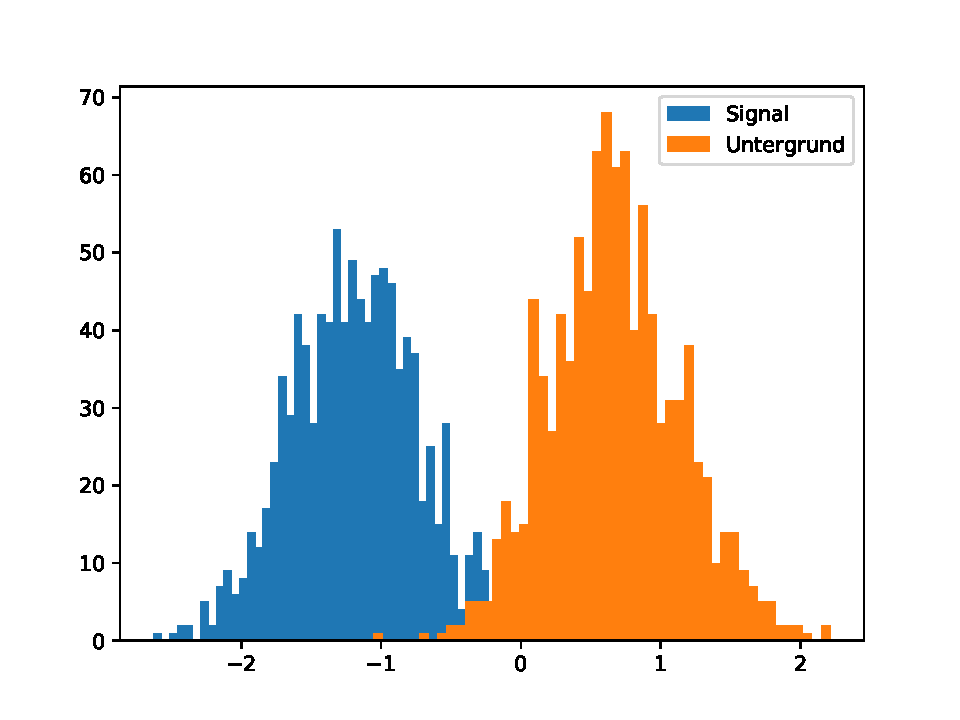
\includegraphics[height=7cm]{hist.pdf}
      \caption{Histogramme der Verteilungen $P_0$ und $P_1$.}
      \label{fig:hist}
    \end{figure}

    \subsection{Aufgabe 12e}

    \begin{figure}[H]
      \centering
      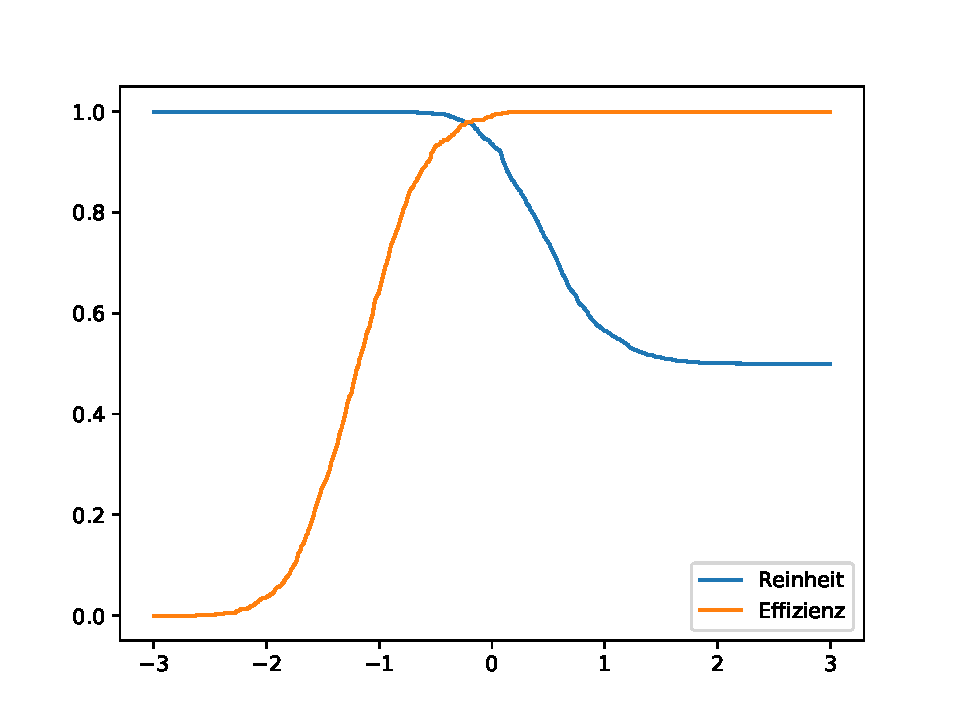
\includegraphics[height=7cm]{reinheit.pdf}
      \caption{Darstellung der Reinheit und Effizienz in Abhängigkeit des Schnittes $\lambda$.}
      \label{fig:reinheit}
    \end{figure}



\end{document}
